
   %%%%%%%%%%%%%%%%%%%%%%%
 %%%  NOAH'S SUPER COOL  %%%
%%%%      ACADEMIC       %%%%
 %%%   LATEX TEMPLATE    %%%
   %%%%%%%%%%%%%%%%%%%%%%%

\documentclass[12pt]{article}
\usepackage[letterpaper]{geometry}
\geometry{top=1in, bottom=1in, left=1in, right=1in}
\usepackage{amsmath}
\usepackage{fontspec}
\usepackage{tgtermes}
\usepackage{hanging}
\usepackage{gensymb}
\setmainfont[
 ItalicFont={texgyretermes-italic.otf},
 BoldFont={texgyretermes-bold.otf},
 ]{texgyretermes-regular.otf}
\usepackage{setspace}
\doublespacing
\usepackage{graphicx}
\graphicspath{ {./graphics/} }

\begin{document}

% Title Page
\pagenumbering{gobble} % remove page numbers
\begin{center}
\topskip0pt
\vspace*{\fill}
Heat Transfer by Radiation \\ Lab 14 - Noah Dinan \\ PHY 1110 - Mayer \\ \today \\
\vspace*{\fill}
\end{center}

\newpage
\pagenumbering{arabic} % resume page numbering
\setlength{\parindent}{0in}

\textbf{Results}\vspace{1em}

After configuring the equipment and setup as defined in the lab instructions, we measured the
room temperature resistance of the lightbulb filament and found it to be $15.9 \Omega$.

Running through the experiment, varying the input voltage using the Variac, we created the data
table below.

\begin{center}
    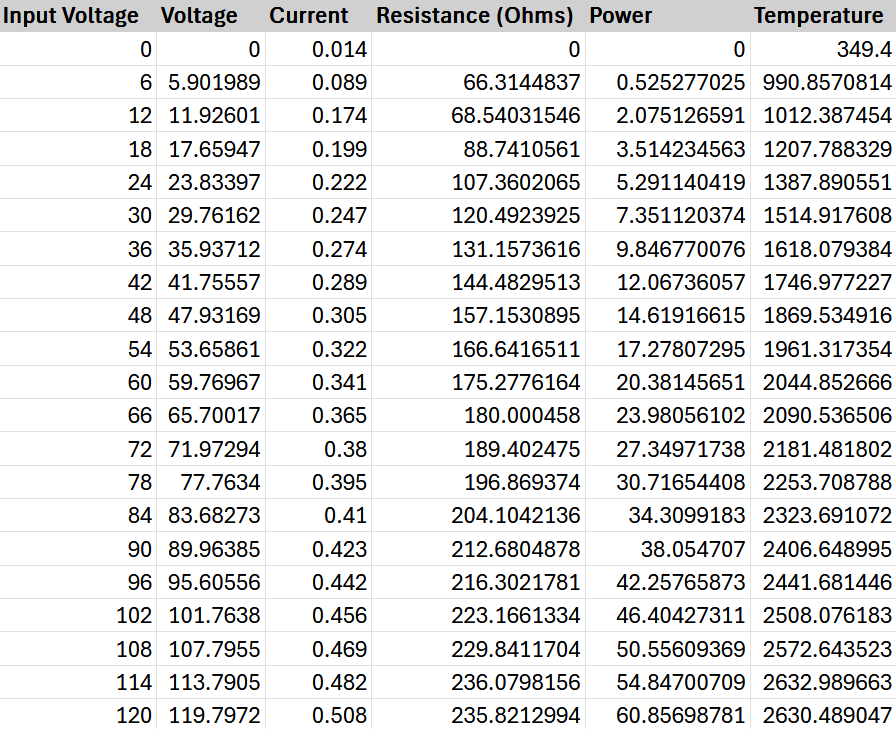
\includegraphics[scale=0.5]{table_14.png}
\end{center}

Graphing the natural log of Power and Temperature from this table then produced the following graph.

\begin{center}
    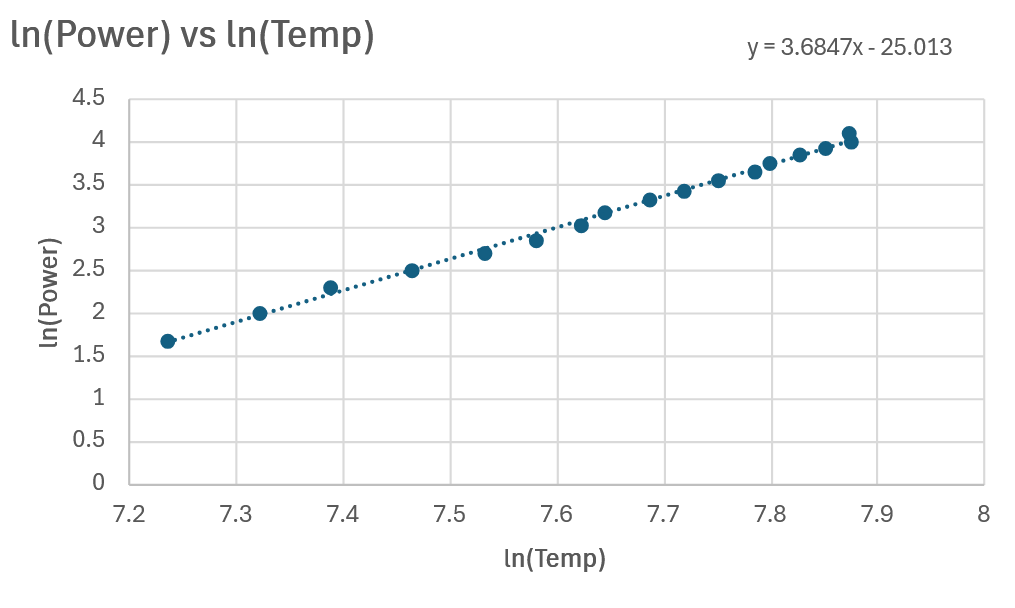
\includegraphics[scale=0.5]{graph_14.png}
\end{center}

We can analyze the slope of this graph and see that it is $3.6847$ which is somewhat close to the expected
value of $4$. This expected value is four due to the following equation for Stefan's Law.

\[ P = \sigma eAT^{4} \]

Our error in this experiment was likely due to the fact that we initially had our multimeter
set to measure DC Voltage and had to convert all of our voltage measurements from DC to AC. This
may have caused some loss in accuracy.

\newpage

\textbf{Conclusions}\vspace{1em}

Our value of $3.6847$ is fairly close to the expected value of $4$, using our value we can also measure the
surface area of our tungsten filament. Using $e = 0.23$, and a y-intercept of 1.5 Watts we solved for A.

\[ A = \frac{P}{\sigma eT^{3.6847}} \]

resulting in a surface area of

\[ A = 1.03 mm^{2} \]

which seems overly low for our filament but was likely due to the error in our measurement of the exponent

\end{document}
